% -*- mode: latex; -*- mustache tags:  
\documentclass[10pt,twoside,english]{_support/latex/sbabook/sbabook}
\let\wholebook=\relax

\usepackage{import}
\subimport{_support/latex/}{common.tex}

%=================================================================
% Debug packages for page layout and overfull lines
% Remove the showtrims document option before printing
\ifshowtrims
  \usepackage{showframe}
  \usepackage[color=magenta,width=5mm]{_support/latex/overcolored}
\fi


% =================================================================
\title{A PharoThings Tutorial}
\author{Allex Oliveira}
\series{Square Bracket tutorials}

\hypersetup{
  pdftitle = {A PharoThings Tutorial},
  pdfauthor = {Allex Oliveira},
  pdfkeywords = {IoT, Raspberry, PharoThings, Pharo}
}


% =================================================================
\begin{document}

% Title page and colophon on verso
\maketitle
\pagestyle{titlingpage}
\thispagestyle{titlingpage} % \pagestyle does not work on the first one…

\cleartoverso
{\small

  Copyright 2017 by Allex Oliveira.

  The contents of this book are protected under the Creative Commons
  Attribution-ShareAlike 3.0 Unported license.

  You are \textbf{free}:
  \begin{itemize}
  \item to \textbf{Share}: to copy, distribute and transmit the work,
  \item to \textbf{Remix}: to adapt the work,
  \end{itemize}

  Under the following conditions:
  \begin{description}
  \item[Attribution.] You must attribute the work in the manner specified by the
    author or licensor (but not in any way that suggests that they endorse you
    or your use of the work).
  \item[Share Alike.] If you alter, transform, or build upon this work, you may
    distribute the resulting work only under the same, similar or a compatible
    license.
  \end{description}

  For any reuse or distribution, you must make clear to others the
  license terms of this work. The best way to do this is with a link to
  this web page: \\
  \url{http://creativecommons.org/licenses/by-sa/3.0/}

  Any of the above conditions can be waived if you get permission from
  the copyright holder. Nothing in this license impairs or restricts the
  author's moral rights.

  \begin{center}
    
\includegraphics[width=0.2\textwidth]{_support/latex/sbabook/CreativeCommons-BY-SA.pdf}
  \end{center}

  Your fair dealing and other rights are in no way affected by the
  above. This is a human-readable summary of the Legal Code (the full
  license): \\
  \url{http://creativecommons.org/licenses/by-sa/3.0/legalcode}

  \vfill

  % Publication info would go here (publisher, ISBN, cover design…)
  Layout and typography based on the \textcode{sbabook} \LaTeX{} class by Damien
  Pollet.
}


\frontmatter
\pagestyle{plain}

\tableofcontents*
\clearpage\listoffigures

\mainmatter

\chapter{Lesson 3 – A brief introduction to Pharo object-oriented language}
Pharo is a new generation reflective language and programming environment. The last code was executed inside the remote inspector. To get started using OOP (Object-Oriented Programming) with classes, methods, and instances, I invite you to implement a simple application to blink the LEDs.
\section{Developing a simple LED blinker}
The following part of this chapter and application was based on the exercise \textcode{Developing a Simple Counter}, of Week 1 of Pharo MOOC (https://mooc.pharo.org/). I strongly recommend that you read and do the \symbol{34}counter exercise\symbol{34} to better understand the concepts explained here. And, of course, do the MOOC to learn how to develop using Pharo and the OOP concept.
\section{Our use case}
We want to create a blinker LED using a few parameters such as time to repeat the blinking LED and how many seconds to wait between blinks. The following code should run in the playground when we finish this lesson:

\begin{displaycode}{plain}
|blinker|
blinker := Blinker new.
blinker timesRepeat: 10 waitForSeconds: 1.
\end{displaycode}

Here is a short explanation of this code:

\begin{itemize}
\item In the first line, we declare the variable \textcode{blinker}. We can use any name. We will use this variable to create an object using the Blinker class;
\item In the second line, we instantiate the Blinker class (with uppercase B) in the \textcode{blinker} variable, creating an object. In this lesson, we will create this class and methods to control the LED;
\item In the third line, we send some messages to the \textcode{blinker} object, for how long and how many times per second. This will make the GPIO behave according to the parameters sent.
\end{itemize}

Now we will develop all the mandatory class and methods to support this scenario.
\section{Create your own class remotely}
Let's create our first class. To create a class in Pharo, we need first to create a package. Inside the package, you can create many classes and inside the classes, you can create many methods. The methods are organized in protocols, to become more easily navigate between them. Take a look in Figure \ref{RemoteBrowser} to better understanding. *edit image, put name in windows

In your local playground, call the Remote System Browser of your Raspberry Pi. If you are already connected to your Raspberry Pharo, you do not need to run the first line below again. This will open a window as shown in Figure \ref{RemoteBrowser} 


\begin{figure}

\begin{center}
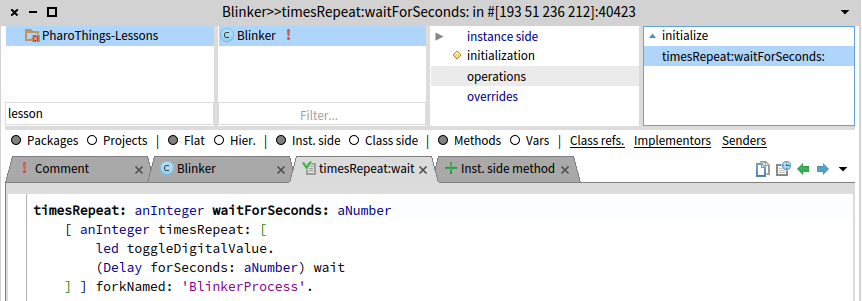
\includegraphics[width=1.0\textwidth]{/Users/allexoliveira/PharoThingsBook/Booklet-APharoThingTutorial/_result/pdf/Chapters/Chap4IntroductiontoPharoOOP/figures/pharothings-remote-system-browser.png}\caption{Remote System Browser.\label{RemoteBrowser}}\end{center}
\end{figure}


\begin{displaycode}{plain}
remotePharo := TlpRemoteIDE connectTo: (TCPAddress ip: #[193 51 236 212] port: 40423).
remotePharo openBrowser.
\end{displaycode}
\section{Create a package}
Let's create a package using the Remote Browser. Right-click the package area and enter the package name, as shown in Figure \ref{CreatingPackage}. In this example, we will create a package named \textcode{PharoThings-Lessons}.


\begin{figure}

\begin{center}
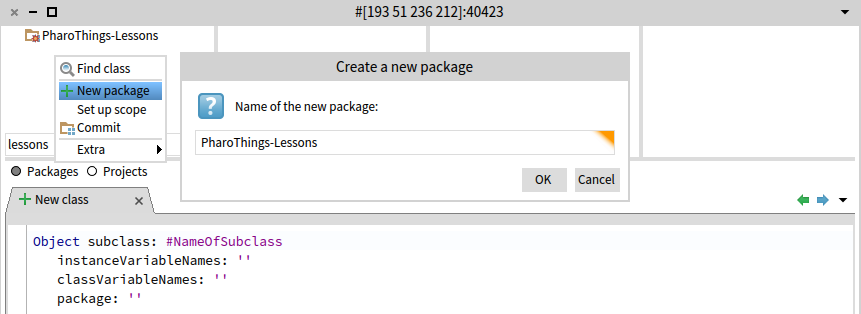
\includegraphics[width=1.0\textwidth]{/Users/allexoliveira/PharoThingsBook/Booklet-APharoThingTutorial/_result/pdf/Chapters/Chap4IntroductiontoPharoOOP/figures/pharothings-creating-package.png}\caption{Creating a package remotely.\label{CreatingPackage}}\end{center}
\end{figure}

\section{Create a class}
To create a new class, edit the default class template by changing the \#NameOfSubclass to the name of the new class. In this example let's create the class \textcode{\#Blinker}. Take care that the class name begins with a capital letter and that you do not remove the hash symbol (\#) in front of NameOfSubClass. 

You must then fill in the names of the instance variables for this class. We need an instance variable called \textcode{led}. Be careful to leave the string quotes!

\begin{displaycode}{plain}
Object subclass: #Blinker
  instanceVariableNames: 'led'
  classVariableNames: ''
  package: 'PharoThings-Lessons'
\end{displaycode}

Now we need to compile it. Right click on the code area and select Accept option. The \textcode{Blinker} class is now compiled and added to the system, as shown in Figure \ref{CreatingClass}.


\begin{figure}

\begin{center}
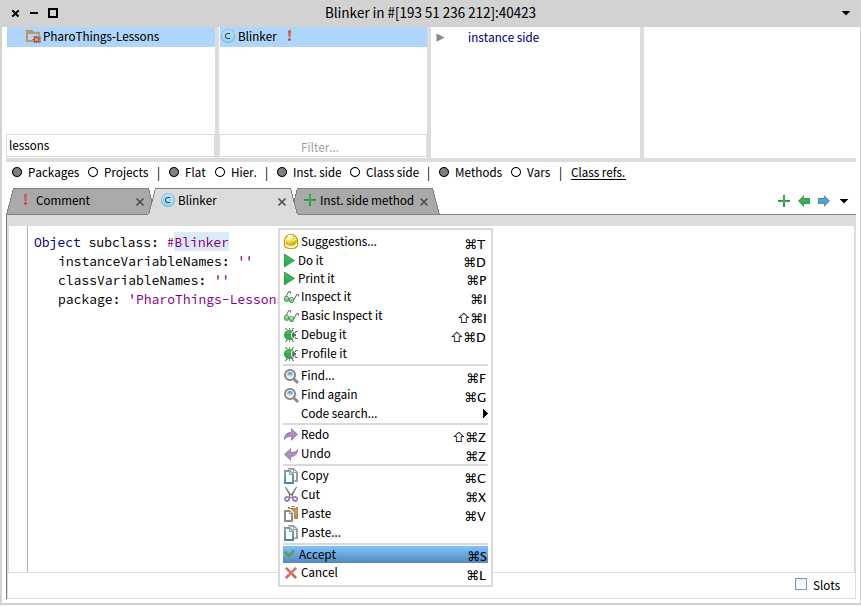
\includegraphics[width=1.0\textwidth]{/Users/allexoliveira/PharoThingsBook/Booklet-APharoThingTutorial/_result/pdf/Chapters/Chap4IntroductiontoPharoOOP/figures/pharothings-creating-class}\caption{Creating a class remotely.\label{CreatingClass}}\end{center}
\end{figure}

\section{Create a protocol}
Let's create a new protocol to organize the methods. The first protocol we are going to create is \textcode{initialization}, as shown in Figure \ref{CreatingProtocol}.


\begin{figure}

\begin{center}
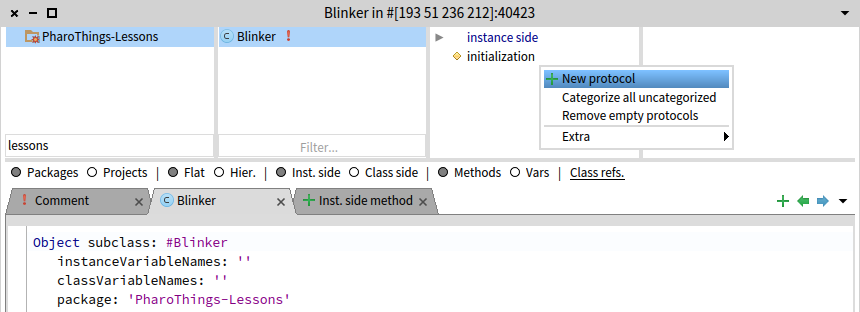
\includegraphics[width=1.0\textwidth]{/Users/allexoliveira/PharoThingsBook/Booklet-APharoThingTutorial/_result/pdf/Chapters/Chap4IntroductiontoPharoOOP/figures/pharothings-creating-protocol}\caption{Creating a package remotely.\label{CreatingProtocol}}\end{center}
\end{figure}

\section{Creating an initialize method}
Inside this protocol, we will create an \textcode{initialize} method. This means that every time we create a new object using this class, in this case, the Blinker class, this method will be executed to define some variable in the new object.

Let's use the instance variable \textcode{led}, which we defined when we created the class. The instance variable is private to the object and accessible by any methods inside this class. These methods can access this variable to get or set any value to it.

\begin{displaycode}{plain}
initialize 
  led := PotClockGPIOPin id: 4 number: 7. 
  led board: RpiBoard3B current; beDigitalOutput
\end{displaycode}

Here is a short explanation of this code:

\begin{itemize}
\item The first line defines the name of the method;
\item In the second line, we configure the GPIO that we wanna use. Note that we need the GPIO number and ID. The ID is required to communicate with Wiring Pi Library. You can see the \textcode{ID} and \textcode{GPIO number} in PotRemoteBoard inspector, as shown in Figure \ref{RemoteInspector};
\item In the third line, we define the model of the Raspberry board and configure this GPIO as beDigitalOutput. This means that when the GPIO change to value:1, the power will go out of the GPIO to power the LED.
\end{itemize}


\begin{figure}

\begin{center}
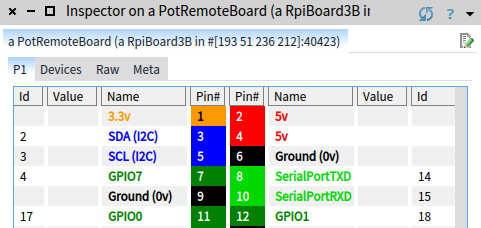
\includegraphics[width=0.7\textwidth]{/Users/allexoliveira/PharoThingsBook/Booklet-APharoThingTutorial/_result/pdf/Chapters/Chap4IntroductiontoPharoOOP/figures/pharothings-board-inspector-id-number.png}\caption{Looking for ID and GPIO number on Remote Inspector.\label{RemoteInspector}}\end{center}
\end{figure}


Compile your code (cmd + S) and the method will be shown in the remote browser, as shown in Figure \ref{InitializeMethod}:


\begin{figure}

\begin{center}
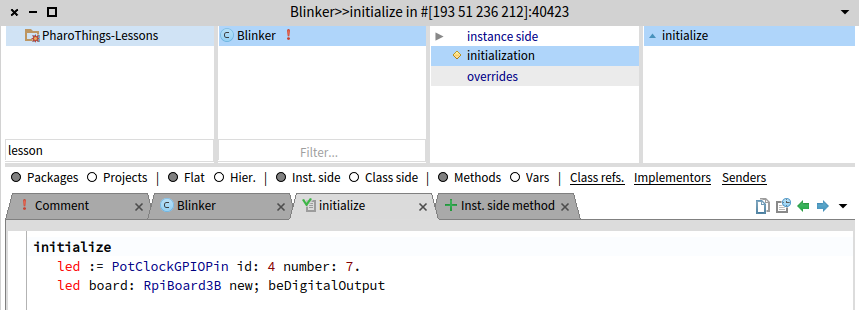
\includegraphics[width=1.0\textwidth]{/Users/allexoliveira/PharoThingsBook/Booklet-APharoThingTutorial/_result/pdf/Chapters/Chap4IntroductiontoPharoOOP/figures/pharothings-creating-method-initialize.png}\caption{Creating the initialize method.\label{InitializeMethod}}\end{center}
\end{figure}

\subsection{Creating a method to do actions}
Now let's create a method to control the object led inside the class Blinker. Let's take the code that we used in PotRemoteBoard inspector to do the LED to blink and replace the numbers on code for two arguments. Create the protocol \textcode{operations} and inside this protocol, create the following method:

\begin{displaycode}{plain}
timesRepeat: anInteger waitForSeconds: aNumber
    [ anInteger timesRepeat: [  
        led toggleDigitalValue. 
        (Delay forSeconds: aNumber) wait  
    ] ] forkNamed: 'BlinkerProcess'.
\end{displaycode}

Here is a short explanation of this code:

\begin{itemize}
\item In the first line, we define the message with timesRepeat: and waitForSeconds:. We inform the kind of value will be received, creating 2 variables: aNumber and anInteger;
\item We replace these variables in the code and now we have the control to say how many times repeat and for how many seconds;
\item We finished the code by putting everything inside a fork to create a process in Pharo. While the process is running, you can open the Remote Process Browser (remotePharo openProcessBrowser) and see the process. This is useful when you wanna kill the remote process.
\end{itemize}

Compile your code (cmd + S) and  the method will be shown in the remote browser, as shown in Figure \ref{OperationsMethod}:


\begin{figure}

\begin{center}
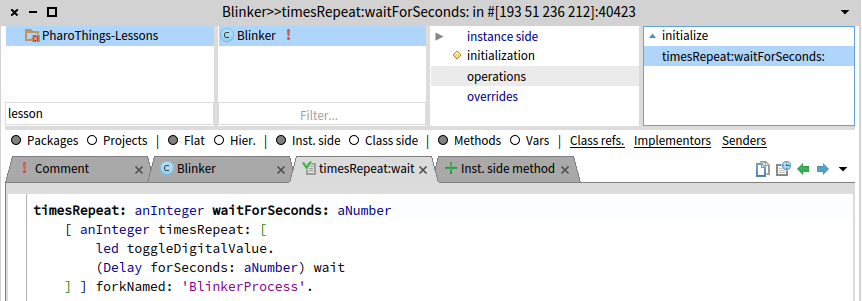
\includegraphics[width=1.0\textwidth]{/Users/allexoliveira/PharoThingsBook/Booklet-APharoThingTutorial/_result/pdf/Chapters/Chap4IntroductiontoPharoOOP/figures/pharothings-creating-method-operations.png}\caption{Creating an operation method.\label{OperationsMethod}}\end{center}
\end{figure}

\section{Using your new class}
Now we can use the class that we created, the Blinker class. To do this, let's open the Remote Playground:

\begin{displaycode}{plain}
remotePharo openPlayground.
\end{displaycode}

and run the code that we saw in the begin of this lesson:

\begin{displaycode}{plain}
|blinker|
blinker := Blinker new. 
blinker timesRepeat: 10 waitForSeconds: 1.
\end{displaycode}

Run this code, as shown in Figure \ref{RemotePlayground} and... \textcode{cool}! Now your LED is blinking! And the better, you did this using object-oriented programming! 

 You do not need to change your code every time you wanna change these parameters. Just change the messages you send to the object and it will behave as you want.


\begin{figure}

\begin{center}
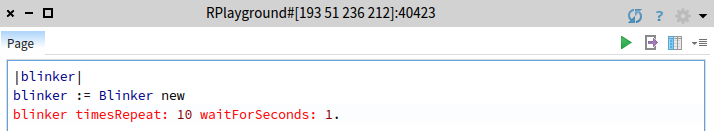
\includegraphics[width=1.0\textwidth]{/Users/allexoliveira/PharoThingsBook/Booklet-APharoThingTutorial/_result/pdf/Chapters/Chap4IntroductiontoPharoOOP/figures/pharothings-remote-playground-blinker.png}\caption{Remote playground.\label{RemotePlayground}}\end{center}
\end{figure}



\section{Save your work}
Don't forget to save your work remotely. To do this, run this command on your local playground:

\begin{displaycode}{plain}
remotePharo saveImage.
\end{displaycode}
\section{Conclusion}
In this tutorial, you learned how to define packages, classes, and methods. The flow of programming that we chose for this first tutorial is similar to most of the programming languages.

With PharoThings you can remotely develop and manage your Raspberry GPIOs. Very easy and powerful.

In the next lesson, let’s use what we learned in this lesson and write a simple code to flow lights using 8 LEDs.



% lulu requires an empty page at the end. That's why I'm using
% \backmatter here.
\backmatter

% Index would go here

\end{document}
